\documentclass{report}

%Para ponerlo en español:
\usepackage[T1]{fontenc}
\usepackage[spanish]{babel}

%para poder citar
\usepackage[backend=biber]{biblatex}
\bibliography{bibliografía.bib}
%\addbibresource{bibliografía.bib}
%\usepackage{csquotes}

%Para poder añadir imágenes:
\usepackage{graphicx}

% Title Page (ya no es necesario)
\title{Proyecto: Interfaz para un filtro de señal cardiaca}
\author{Caballero Trinidad Flor Isabel. \\ Cortés Ramírez Samuel Jefte. \\ García García Ian Pablo. \\ Pérez Roldan Eduardo Alejandro. \\ Cabañas Alba Alejandro. \\ Alfonso Gamboa Rubén.}


\begin{document}

%Portada
\begin{titlepage}
	\centering
	{
\includegraphics[width=0.2\textwidth]{recursos/Universidad_Veracruzana}\par}
	\vspace{1cm}
	{\bfseries\LARGE Universidad Veracruzana \par}
	\vspace{1cm}
	{\scshape\Large Ingeniería Biomédica \par}
	\vspace{3cm}
	{\scshape\Huge Interfaz para un filtro de frecuencia cardiáca. \par}
	\vspace{2cm}
	{\itshape\Large Proyecto. \par}
	\vfill
	{\Large Autores: \par}
	{\Large Caballero Trinidad Flor Isabel. \\ Cortés Ramírez Samuel Jefte. \\ García García Ian Pablo. \\ Pérez Roldan Eduardo Alejandro. \\ Cabañas Alba Alejandro. \\ Alfonso Gamboa Rubén. \par}
	\vfill
	
\end{titlepage}

%\tableofcontents
\chapter{Parcial 1}
	\section{keywords}
	Frecuencia cardaica, Interfaz, Filtro de frecuencia cardaiaca, Interfaz para un filtro, SPython, Interfaz Médica, Ingeniería Biomédica, Arduino.
	
	\section{Introducción.}
		El siguiente proyecto tiene como finalidad responder a la pregunta ¿Cómo desarrollar una interfaz que facilite la visualización y procesamiento de datos de la frecuencia cardiaca?, teniendo como principal objetivo visualizar la frecuencia cardiaca del usuario mediante una interfaz a partir del lenguaje de programación Python \cite{python3}. 
		
		Los temas que se abordaran y se trabajaran para la realización óptima del proyecto son: desarrollar una interfaz amigable con el usuario con la finalidad de interpretar los datos de manera precisa, garantizando la funcionalidad del sistema diseñando una interfaz para una gráfica; con el lenguaje de programación Python se busca lograr leer y escribir ficheros, desarrollar un código legible para el programador y crear una base de datos (con de ayuda de sql \cite{SQL}) para los datos recolectados, con el propósito de calcular la media aritmética para añadir funcionalidad que permita al usuario calcular su recuperación cardiaca. Este proyecto esta dirigido a un público general busca monitorear su frecuencia cardiaca.  
		
		Se llevará a cabo el proyecto con la finalidad de adquirir conocimiento sobre la creación de una interfaz en el lenguaje de programación Python, con la ayuda de una practica anterior relacionada a la Ingeniería Biomédica, se obtendrán lecturas de medición para la realización de prueba predictiva en índices para medir la salud cardiaca, se diseñara una versión base de una interfaz para el almacenamiento de señales biomédicas, con la finalidad de utilizarlas en un futuro y poder manipularlas, también se trabajara en conjunto con compañeros de la carrera de Instrumentación Electrónica, para así reforzar el trabajo en equipo y crear un frontend y un backend. 
		
		Para filtrar la búsqueda de la información necesaria para poder realizar el proyecto, se procedió a una búsqueda sistematizada de evidencia siguiendo los criterios de inclusión: artículos, libros, tesis, publicadas desde el año 1990 hasta la actualidad, información relacionada a como crear una interfaz en el lenguaje de programación Python, información del funcionamiento y características de la frecuencia cardiaca. 
		
		En esta sección se elabora una revisión bibliográfica de los conceptos generales a partir de los cuales se sustenta este proyecto, los conceptos a considerar son: señales biomédicas, interfaz, base de datos, frontend, backend, lenguaje de programación Python, frecuencia cardiaca.
		
		\paragraph{Señales biomédicas.} ¿Qué es una señal biomédica? "Las señales biomédicas representan variables fisiológicamente relevantes de las que nos interesa su curso temporal. La variable puede ser un voltaje muy pequeño, como el electroencefalograma, o algunos órdenes de magnitud mayor, como el electrocardiograma, o puede ser una variable que originalmente no es eléctrica, como la presión o la temperatura"\cite{biomedica_s}. 
		\paragraph{Interfaz.} ¿Qué es una interfaz? la RAE la define como: "Conexión o frontera común entre dos aparatos o sistemas independientes, quepermite el intercambio de información o la coordinación de sus funciones." \cite{rae_interfaz}
		\paragraph{Base de datos.} ¿Qué es una base de datos?, Una base de datos es una recopilación de archivos dedicados a guardar informaciónentre sí, es decir, que pertenecen al mismo contexto; estos datos serán usados afuturo en diferentes tareas, además, pueden ser visualizados y utilizados por más deuna persona \cite{BaseDDatos}
		\paragraph{Frontend y backend.} ¿Qué es front-end y back-end?. El front-end es la parte que va a interactuar con el usuario, en el caso de nuestroproyecto será la interfaz, el back-end es la parte que contiene la infraestructura quele va a dar funcionalidad a el proyecto. \cite{FrontendBackend}
		\paragraph{Lenguaje de programación Python.} Python es un lenguaje de progamación de alto nivel, el cual ha agarrado bastante popularidad en nuestros tiempos gracias a su legibilidad, razón por la cual también es el más usado en cuanto a aprender a programar se refiere; razón por la cual hoy en dia contamos con un sin fin de librerías y documentación al respecto. \cite{python3}
		\paragraph{Frecuencia cardiaca.} La frecuencia cardiaca o pulso, es la cantidad de veces que late por cierto periodode tiempo, se puede medir en varias partes del cuerpo como la muñeca, cuello,pecho, entre otros. La frecuencia de un adulto suele encontrarse dentro de 60 – 100latidos por minuto.\cite{FrecuenciaCardiaca}
			
	\section{Metodología.}
	Se utilizará el lenguaje de programación Python \cite{python3} para la aplicación principal. Se utilizará la librería “TkInter”\cite{tkinter} para el diseño de unainterfaz "amigable" con el usuario. Para el despliegue de las gráficas de pulso cardiaco se utilizará la librería seaborn de python \cite{Seaborn}.\\
	Para la obtención de las señales cardiacas se utilizará un sensor” Max 30100” y una placa arduino uno con el cual se medirá el pulso cardiaco de una persona; para la comunicación se utilizara un programa por aparte heco en python. Posteriormente guardarlo en un archivo “.txt", dicho archivo pasará por un filtro realizado por nuestros compañeros de instrumentación electrónica para así entregarnos una señal legible y más limpia, con esto podremos hacer la interfaz en Python.\\
	Para una mejor organización y para un control se versiones, se usará git y github. Publicado en: https://github.com/Benchito2003/Proyecto-programacion.git
	
	\subsubsection{Placa Arduino uno}
	\begin{figure}[h]
		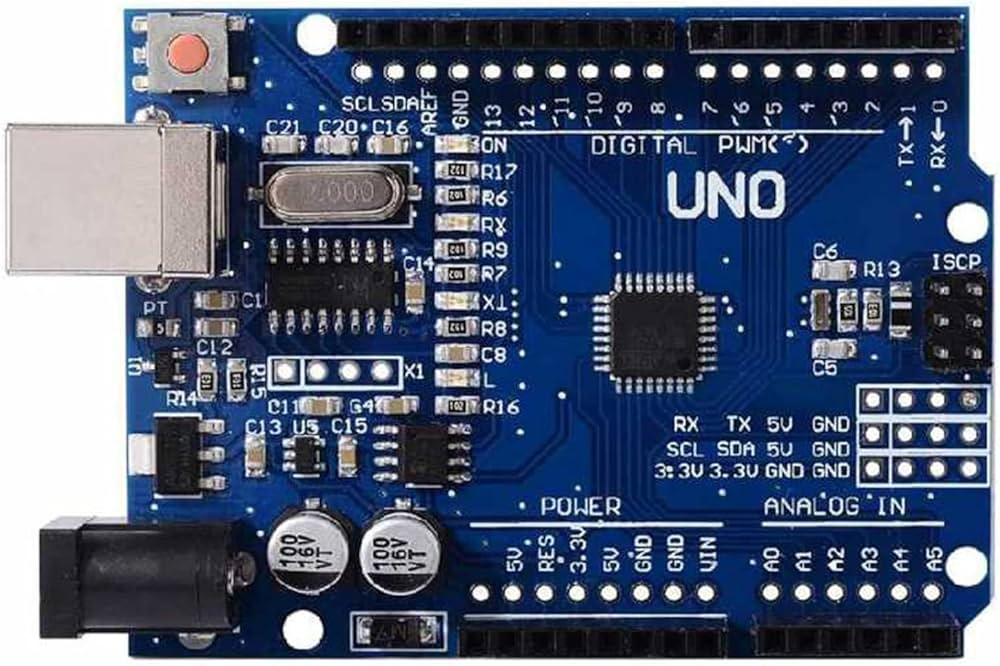
\includegraphics[width=0.5\textwidth]{recursos/placa-arduino} 
	\end{figure}
	
	\subsubsection{Sensor max 30100}
	\begin{figure}[h]
		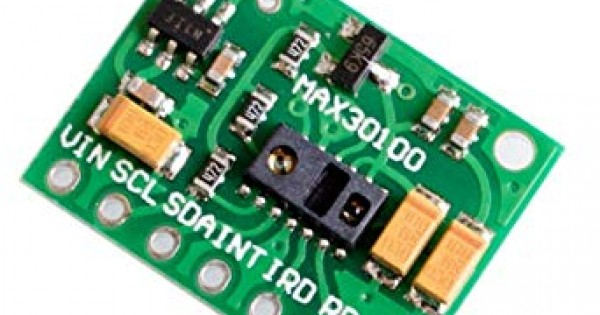
\includegraphics[width=0.5\textwidth]{recursos/imagen}
	\end{figure}
	
	
	\printbibliography
%\begin{abstract}
%\end{abstract}
\end{document}

